% Options for packages loaded elsewhere
\PassOptionsToPackage{unicode}{hyperref}
\PassOptionsToPackage{hyphens}{url}
\PassOptionsToPackage{dvipsnames,svgnames,x11names}{xcolor}
%
\documentclass[
  letterpaper,
  DIV=11]{scrreprt}

\usepackage{amsmath,amssymb}
\usepackage{lmodern}
\usepackage{iftex}
\ifPDFTeX
  \usepackage[T1]{fontenc}
  \usepackage[utf8]{inputenc}
  \usepackage{textcomp} % provide euro and other symbols
\else % if luatex or xetex
  \usepackage{unicode-math}
  \defaultfontfeatures{Scale=MatchLowercase}
  \defaultfontfeatures[\rmfamily]{Ligatures=TeX,Scale=1}
\fi
% Use upquote if available, for straight quotes in verbatim environments
\IfFileExists{upquote.sty}{\usepackage{upquote}}{}
\IfFileExists{microtype.sty}{% use microtype if available
  \usepackage[]{microtype}
  \UseMicrotypeSet[protrusion]{basicmath} % disable protrusion for tt fonts
}{}
\makeatletter
\@ifundefined{KOMAClassName}{% if non-KOMA class
  \IfFileExists{parskip.sty}{%
    \usepackage{parskip}
  }{% else
    \setlength{\parindent}{0pt}
    \setlength{\parskip}{6pt plus 2pt minus 1pt}}
}{% if KOMA class
  \KOMAoptions{parskip=half}}
\makeatother
\usepackage{xcolor}
\setlength{\emergencystretch}{3em} % prevent overfull lines
\setcounter{secnumdepth}{5}
% Make \paragraph and \subparagraph free-standing
\ifx\paragraph\undefined\else
  \let\oldparagraph\paragraph
  \renewcommand{\paragraph}[1]{\oldparagraph{#1}\mbox{}}
\fi
\ifx\subparagraph\undefined\else
  \let\oldsubparagraph\subparagraph
  \renewcommand{\subparagraph}[1]{\oldsubparagraph{#1}\mbox{}}
\fi


\providecommand{\tightlist}{%
  \setlength{\itemsep}{0pt}\setlength{\parskip}{0pt}}\usepackage{longtable,booktabs,array}
\usepackage{calc} % for calculating minipage widths
% Correct order of tables after \paragraph or \subparagraph
\usepackage{etoolbox}
\makeatletter
\patchcmd\longtable{\par}{\if@noskipsec\mbox{}\fi\par}{}{}
\makeatother
% Allow footnotes in longtable head/foot
\IfFileExists{footnotehyper.sty}{\usepackage{footnotehyper}}{\usepackage{footnote}}
\makesavenoteenv{longtable}
\usepackage{graphicx}
\makeatletter
\def\maxwidth{\ifdim\Gin@nat@width>\linewidth\linewidth\else\Gin@nat@width\fi}
\def\maxheight{\ifdim\Gin@nat@height>\textheight\textheight\else\Gin@nat@height\fi}
\makeatother
% Scale images if necessary, so that they will not overflow the page
% margins by default, and it is still possible to overwrite the defaults
% using explicit options in \includegraphics[width, height, ...]{}
\setkeys{Gin}{width=\maxwidth,height=\maxheight,keepaspectratio}
% Set default figure placement to htbp
\makeatletter
\def\fps@figure{htbp}
\makeatother
\newlength{\cslhangindent}
\setlength{\cslhangindent}{1.5em}
\newlength{\csllabelwidth}
\setlength{\csllabelwidth}{3em}
\newlength{\cslentryspacingunit} % times entry-spacing
\setlength{\cslentryspacingunit}{\parskip}
\newenvironment{CSLReferences}[2] % #1 hanging-ident, #2 entry spacing
 {% don't indent paragraphs
  \setlength{\parindent}{0pt}
  % turn on hanging indent if param 1 is 1
  \ifodd #1
  \let\oldpar\par
  \def\par{\hangindent=\cslhangindent\oldpar}
  \fi
  % set entry spacing
  \setlength{\parskip}{#2\cslentryspacingunit}
 }%
 {}
\usepackage{calc}
\newcommand{\CSLBlock}[1]{#1\hfill\break}
\newcommand{\CSLLeftMargin}[1]{\parbox[t]{\csllabelwidth}{#1}}
\newcommand{\CSLRightInline}[1]{\parbox[t]{\linewidth - \csllabelwidth}{#1}\break}
\newcommand{\CSLIndent}[1]{\hspace{\cslhangindent}#1}

\KOMAoption{captions}{tableheading}
\makeatletter
\makeatother
\makeatletter
\@ifpackageloaded{bookmark}{}{\usepackage{bookmark}}
\makeatother
\makeatletter
\@ifpackageloaded{caption}{}{\usepackage{caption}}
\AtBeginDocument{%
\ifdefined\contentsname
  \renewcommand*\contentsname{Inhaltsverzeichnis}
\else
  \newcommand\contentsname{Inhaltsverzeichnis}
\fi
\ifdefined\listfigurename
  \renewcommand*\listfigurename{Abbildungsverzeichnis}
\else
  \newcommand\listfigurename{Abbildungsverzeichnis}
\fi
\ifdefined\listtablename
  \renewcommand*\listtablename{Tabellenverzeichnis}
\else
  \newcommand\listtablename{Tabellenverzeichnis}
\fi
\ifdefined\figurename
  \renewcommand*\figurename{Abbildung}
\else
  \newcommand\figurename{Abbildung}
\fi
\ifdefined\tablename
  \renewcommand*\tablename{Tabelle}
\else
  \newcommand\tablename{Tabelle}
\fi
}
\@ifpackageloaded{float}{}{\usepackage{float}}
\floatstyle{ruled}
\@ifundefined{c@chapter}{\newfloat{codelisting}{h}{lop}}{\newfloat{codelisting}{h}{lop}[chapter]}
\floatname{codelisting}{Listing}
\newcommand*\listoflistings{\listof{codelisting}{Listingverzeichnis}}
\makeatother
\makeatletter
\@ifpackageloaded{caption}{}{\usepackage{caption}}
\@ifpackageloaded{subcaption}{}{\usepackage{subcaption}}
\makeatother
\makeatletter
\@ifpackageloaded{tcolorbox}{}{\usepackage[many]{tcolorbox}}
\makeatother
\makeatletter
\@ifundefined{shadecolor}{\definecolor{shadecolor}{rgb}{.97, .97, .97}}
\makeatother
\makeatletter
\makeatother
\ifLuaTeX
\usepackage[bidi=basic]{babel}
\else
\usepackage[bidi=default]{babel}
\fi
\babelprovide[main,import]{ngerman}
% get rid of language-specific shorthands (see #6817):
\let\LanguageShortHands\languageshorthands
\def\languageshorthands#1{}
\ifLuaTeX
  \usepackage{selnolig}  % disable illegal ligatures
\fi
\IfFileExists{bookmark.sty}{\usepackage{bookmark}}{\usepackage{hyperref}}
\IfFileExists{xurl.sty}{\usepackage{xurl}}{} % add URL line breaks if available
\urlstyle{same} % disable monospaced font for URLs
\hypersetup{
  pdftitle={In Arbeit!! - HWE-Skript},
  pdfauthor={Leopold Götsch},
  pdflang={de},
  colorlinks=true,
  linkcolor={blue},
  filecolor={Maroon},
  citecolor={Blue},
  urlcolor={Blue},
  pdfcreator={LaTeX via pandoc}}

\title{In Arbeit!! - HWE-Skript}
\author{Leopold Götsch}
\date{06.06.23}

\begin{document}
\maketitle
\ifdefined\Shaded\renewenvironment{Shaded}{\begin{tcolorbox}[enhanced, breakable, interior hidden, sharp corners, frame hidden, borderline west={3pt}{0pt}{shadecolor}, boxrule=0pt]}{\end{tcolorbox}}\fi

\renewcommand*\contentsname{Inhaltsverzeichnis}
{
\hypersetup{linkcolor=}
\setcounter{tocdepth}{2}
\tableofcontents
}
\bookmarksetup{startatroot}

\hypertarget{willkommen-zum-skript}{%
\chapter*{Willkommen zum Skript}\label{willkommen-zum-skript}}
\addcontentsline{toc}{chapter}{Willkommen zum Skript}

\markboth{Willkommen zum Skript}{Willkommen zum Skript}

\textbf{In Arbeit!!}

Dieses Skriptum dient zu Unterstützung und Ergänzung der Inhalte aus dem
Unterricht. Der ``rote Faden'' im Unterricht ist in den jeweiligen
Klassennotizbüchern zu finden. Darin sind auch Links zu den passenden
Kapiteln in diesem Skript zu finden. Das Skriptum wird ständig erweitert
und verbessert. Input ist willkommen.

\hypertarget{verbessern}{%
\section*{Verbessern}\label{verbessern}}
\addcontentsline{toc}{section}{Verbessern}

\markright{Verbessern}

Ich freue mich über alle Fehlerkorrekturen und Verbesserungsvorschläge
die mich erreichen. Am einfachsten ist dies via Mail.

\hypertarget{mitwirken}{%
\section*{Mitwirken}\label{mitwirken}}
\addcontentsline{toc}{section}{Mitwirken}

\markright{Mitwirken}

Wer am Skriptum mitarbeiten möchte kann mich gerne kontaktieren. Meine
Kontaktdaten sind auf der Homepage der HTL-Anichstrasse zu finden.

Viel Vergnügen mit HWE und dem interaktiven Quarto Book!

\part{3. Jahrgang}

\hypertarget{der-transistor}{%
\chapter{Der Transistor}\label{der-transistor}}

\hypertarget{feldeffekttransistor}{%
\section{Feldeffekttransistor}\label{feldeffekttransistor}}

Die einfachste und die gleichzeitig eine der wichtigsten Anwendungen des
MOSFET's ist der Schalter. Mittels Spannnung am Gate wird der MOSFET
ein- und ausgeschalten.

\begin{figure}

{\centering 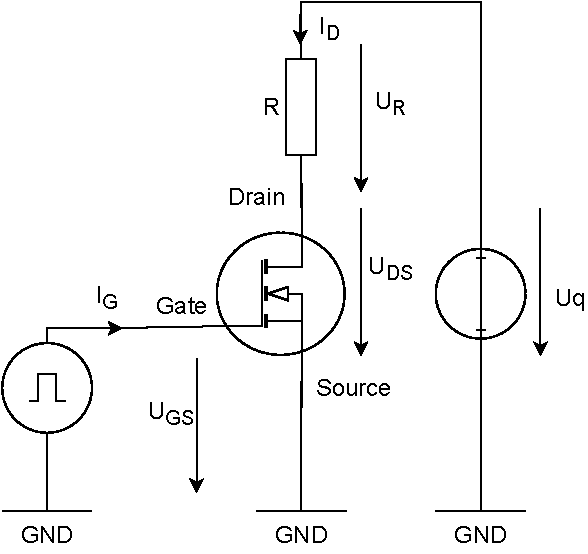
\includegraphics{Transistoren/Grafiken/NChannelenhancementSwitch.pdf}

}

\caption{\label{fig-n-Channel_switch}N-Kanal MOSFET als Schalter}

\end{figure}

Die notwendigen und zulässigen Spannungen sind aus dem Datenblatt des
gewählten Transistors zu entnehmen. Am Gate wird kein Vorwiderstand
benötigt, da der Eingangswiderstand des MOSFET's sehr hoch ist und
dadurch \(I_D = 0 \ \mathrm{A}\) angenommen werden kann.

\hypertarget{aufgabe}{%
\subsection{Aufgabe}\label{aufgabe}}

\hypertarget{teil-1-n-kanal-anreicherungstyp}{%
\subsubsection{Teil 1: N-Kanal
Anreicherungstyp}\label{teil-1-n-kanal-anreicherungstyp}}

Simulieren Sie die Schaltung. Wählen Sie die Spannungen aus dem
Datenblatt aus. Geben Sie für zwei Eingangspulse den Strom durch, und
die Spannung über den Widerstand. Verwenden Sie dafür die
Transientenanalyse und geben Sie deutlich an ob das Ergebnis den
Erwartungen entspricht oder nicht. Argumentieren Sie Ihre Aussage.

\hypertarget{teil-2-p-kanal-anreicherungstyp}{%
\subsubsection{Teil 2: P-Kanal
Anreicherungstyp}\label{teil-2-p-kanal-anreicherungstyp}}

Simulieren Sie die Schaltung erneut unter der verwendung eines P-Kanal
Anreicherungstypen. Passen Sie die Spannungen so an, dass auch dieser
als Schalter funktioniert. Verwenden Sie dazu erneut das passende
Datenblatt. Geben Sie deutlich an ob das Ergebnis den Erwartungen
entspricht oder nicht. Argumentieren Sie Ihre Aussage.

\hypertarget{bipolartransistor}{%
\section{Bipolartransistor}\label{bipolartransistor}}

\hypertarget{die-emitterschaltung-mit-temperaturstabilisierung}{%
\subsection{Die Emitterschaltung mit
Temperaturstabilisierung}\label{die-emitterschaltung-mit-temperaturstabilisierung}}

Ein einfacher Spannungsverstärker. Der Re dient der
Temperaturstabilisierung der \(U_{BE}\) Strecke.

\begin{figure}

{\centering 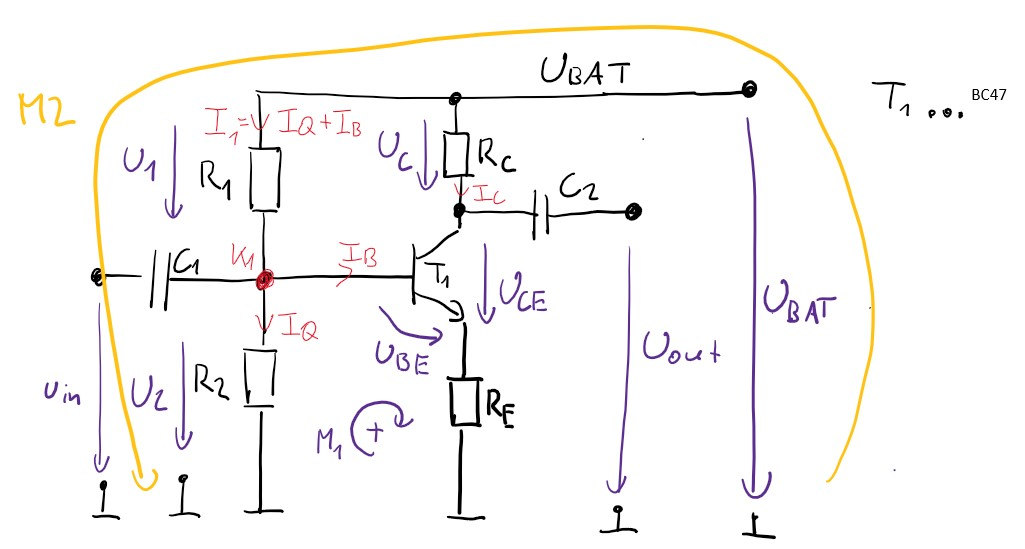
\includegraphics{Transistoren/Grafiken/Emittergrundschaltung_mit_Re.pdf}

}

\caption{\label{fig-BJT_Emitter_mit_Re}Bipolartransistor in
Emittergrundschaltung mit Re}

\end{figure}

\hypertarget{aufgabenstellung}{%
\subsection{Aufgabenstellung}\label{aufgabenstellung}}

Entwerfen Sie einen Spannungsverstärker mit einer Verstärkung.

\begin{equation}\protect\hypertarget{eq-vU_eq}{}{
v_{U} = - \frac{R_{c}}{R_{e}}
}\label{eq-vU_eq}\end{equation}

\(R_{e}\) \ldots{} Widerstand zwischen dem Emitter und der Masse

\(R_{c}\) \ldots{} Widerstand zwischen der Versorgungsspannung und dem
Kollektor

\(v_{U}\) \ldots{} Spannungsverstärkung

\(v_{U}\) = -20\(\ \mathtt{\text{}}\)

\hypertarget{gegeben}{%
\subsubsection{Gegeben}\label{gegeben}}

\hypertarget{aus-der-angabe}{%
\paragraph{Aus der Angabe}\label{aus-der-angabe}}

\(v_{U}\) = -20\(\ \mathtt{\text{}}\)

\(v_{U}\) \ldots{} Spannungsverstärkung

\(U_{bat}\) = 10\(\ \text{V}\)

\(U_{bat}\) \ldots{} Versorgungsspannung

\hypertarget{aus-dem-datenblatt}{%
\paragraph{Aus dem Datenblatt}\label{aus-dem-datenblatt}}

\(B\) = 300\(\ \mathtt{\text{}}\)

\(B\) \ldots{} Stromverstärkung, \(h_{fe}\)

\hypertarget{aus-der-erfahrung-faustregel}{%
\paragraph{Aus der Erfahrung /
Faustregel}\label{aus-der-erfahrung-faustregel}}

\begin{itemize}
\tightlist
\item
  Zahlenwerte
\end{itemize}

\(U_{T}\) = 0.025\(\ \text{V}\)

\(U_{T}\) \ldots{} Temperaturspannung

\(I_{c}\) = 0.001\(\ \text{A}\)

\(I_{c}\) \ldots{} Strom in den Kollektor

\(U_{BE}\) = 0.7\(\ \text{V}\)

\(U_{BE}\) \ldots{} Spannungsabfall zwischen Basis und Emitter

\begin{itemize}
\tightlist
\item
  Gleichungen
\end{itemize}

\begin{equation}\protect\hypertarget{eq-Ic1}{}{
I_{c} = \frac{U_{bat}}{2 R_{c} + 2 R_{e}}
}\label{eq-Ic1}\end{equation}

\(U_{bat}\) \ldots{} Versorgungsspannung

\(R_{c}\) \ldots{} Widerstand zwischen der Versorgungsspannung und dem
Kollektor

\(I_{c}\) \ldots{} Strom in den Kollektor

\(R_{e}\) \ldots{} Widerstand zwischen dem Emitter und der Masse

\hypertarget{berechnung}{%
\subsection{Berechnung}\label{berechnung}}

\begin{itemize}
\tightlist
\item
  Gleichung Gleichung~\ref{eq-vU_eq} nach \(R_e\) auflösen. Das Ergebnis
  in Gleichung Gleichung~\ref{eq-Ic1} einsetzen und nach \(R_c\)
  auflösen.
\end{itemize}

\begin{equation}\protect\hypertarget{eq-Re1}{}{
v_{U} = - \frac{R_{c}}{R_{e}}
}\label{eq-Re1}\end{equation}

\[
I_{c} = \frac{U_{bat}}{2 R_{c} - \frac{2 R_{c}}{v_{U}}}
\]\{\#Ic\_eq2\}

\begin{equation}\protect\hypertarget{eq-Rc1}{}{
R_{c} = \frac{U_{bat} v_{U}}{2 I_{c} \left(v_{U} - 1\right)}
}\label{eq-Rc1}\end{equation}

\(R_{c}\) = 4761.90476190476\(\ \Omega\)

\hypertarget{die-kollektorgrundschaltung}{%
\subsection{Die
Kollektorgrundschaltung}\label{die-kollektorgrundschaltung}}

\bookmarksetup{startatroot}

\hypertarget{references}{%
\chapter*{References}\label{references}}
\addcontentsline{toc}{chapter}{References}

\markboth{References}{References}

\hypertarget{refs}{}
\begin{CSLReferences}{0}{0}
\end{CSLReferences}



\end{document}
